\chapter{Xcore Approach}\label{ch:2}

\epigraph{Programming today is a race between software engineers striving to
build bigger and better idiot-proof programs, and the Universe trying to produce
bigger and better idiots. So far, the Universe is winning.}{Rich Cook}

        For the problems mentioned in the above chapters we have implemented a tool called XCore.
As we shall see in the following sections, our tools uses annotations and interfaces in order for developers
to express their meta-model for the analysis tools in a type safe maner. Based on the expressed meta-model
we generate the appropriate code for it.
        In order to evaluate the application we have also reimplemented a front-end tool called InsiderView 
\cite{tools:iPlasma} which allows you to integrate different  metrics based on the meta-metamodel from CodePro.
In our case, Insider becomes a generic Eclipse UI for tools developed using XCore.

\section{Related Work}
       
        In essence XCore is a tool for meta-programming. It contains meta-meta-model which allows the user to describe any meta-model respecting the constraints. Thus is bears some similarity
 with other tools which try to solve the problems metioned above, like it such as:
                \begin{description}[labelindent=2cm]
                        \item[Rascal] \cite{tools:rascal}
                        \item[Soot] \cite{tools:soot}
                        \item[Fame] \cite{tools:fame}
                \end{description}
        Rascal is a meta-model programming language. It allows a user to express any meta-model for the development / integration of analysis tools. To the best of my knowledge there is no way
to interact wit other concrete meta-models like those from Wala and Jdt. This is one of it's major disadvantage, another being the time and resources need to fully learn the language before using
it. In the case of XCore, one only needs to know the Java programming language and to understand the basic and a few XCore concepts.  Also, at time of writing, there is also the problem of running time. 
According to \cite{tools:rascal} the runtime environment is pretty slow.

        Soot is Java framework developed for code analysis. It directly analyzes jvm bytecode and can represent in several low level representations. Unlinke XCore, which provides support for 
high analysis tools, the goal of the framework is to provide the necessary tools in order to develope optimization for applications. Also, to the best of my understanding Soot is limited to the
analysis of Java byte code, whereas XCore can integrate with and language library backend, provided that the library is written in Java (or C and which can be integrated in Java applications).

        Fame is similar in scope and idea of development with XCore. It uses the FM3 meta-meta-mode \cite{tools:fame} and which is handeled by the JavaFame Tool. The meta-model for the developed
tool is described in a msfe in file. By contract, XCore allows de developers to describe the meta-mode directly in the Java source by use of annotations. The main disadvantage in using external
files in order to provide configurations is the lack of support for refactorings (i.e refactoring the XCore meta-model is clearly reflected in code, which the compiler can type check. Refactoring
done on the Fame meta-mode which is in an external msf file cannot be checked and bugs and incompatibilites my appear). 



\section {Solution Overview}\label{ch:2.1}

        In Figure \ref{fig:XCoreSystem} we can see the basic architecture of the XCore system. There are three main components to this
system:
        \begin{itemize}
                \item Annotation Component
                \item Interface Component
                \item Annotation Processor
        \end{itemize}
        
        \begin{figure}
        \centering
        \scalebox{0.4}{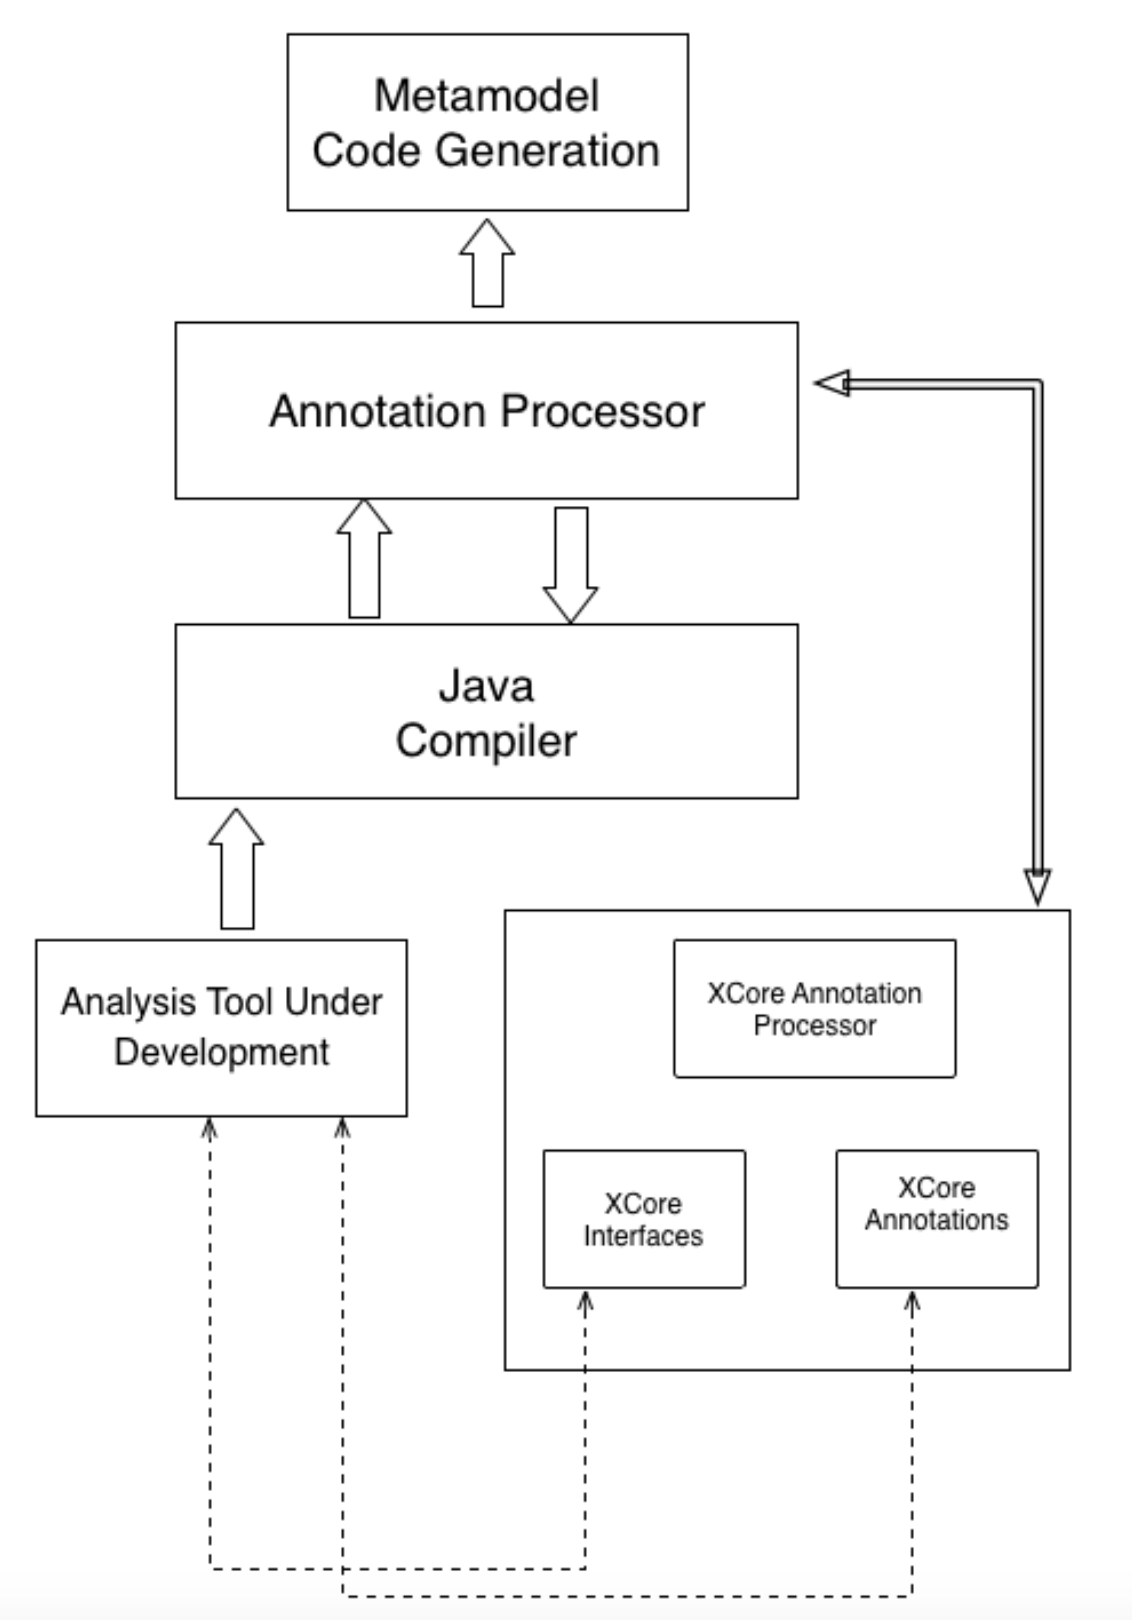
\includegraphics{../img/solution/XCorexSystem.png}}
        \caption{XCorex System overview \cite{oldThesis}}
        \label{fig:XCoreSystem}
        \end{figure}

\subsection{Annotation Component}\label{ch:2.1.1}
        
        The annotation component, as you might have guessed, provides the necessary annotations in order to describe the meta-model.
Annotations are used as markers to identify the components of the analysis tool and also to distinguish between diferent types of entities and thier relationships as described below.
This is only half the story, we also use interfaces, described in the section below \ref{ch:2.1.2}, to insure the type safety of the meta-model, and uniformity 
between similar components.

        As it can be seen from the code below, the {J}ava annotations are allowed only on concrete types, i.e classes. 

\small
\begin{lstlisting}[language=Java, numbers=left]
@Target(ElementType.TYPE)
public @interface RelationBuilder {}   
\end{lstlisting}
\normalsize{} \label{codeSection:RelationBuilder}
                          
\small
\begin{lstlisting}[language=Java,numbers=left]
@Target(ElementType.TYPE)
public @interface PropertyComputer {}
\end{lstlisting}
\normalsize{} \label{codeSection:PropertyComputer} 

\small
\begin{lstlisting}[language=Java, numbers=left]
@Target(ElementType.TYPE)
public @interface ActionPerformer {}
\end{lstlisting}
\normalsize{} \label{codeSection:ActionPerformer} 


        In Figure \ref{fig:XMetaModel} we can see the design of the meta-meta-model in the left part, which is based on the conceptual meta-meta-model described
by Ganea et al \cite{paper:ganea}. In the right part we can see an example of a meta-model that can be described (ie. an instantiation of the meta-meta-model). 

        XMethod and XClass represent \textit{entities} of the meta-model which describe methods and classes. Any entity has certain \textit{properties} which represent
result of analysis. For example \textit{NoOfArgsComputer} represents a \textit{property } associated to an \textit{entity}, in this case the XMethod \textit{entity}.
Besides properties, we can express an relationship between entities. In our case, a we have a inclusion relationship, an XClass includes multiple XMethod elements. This can
be easily seen that is represented by the \textit{MethodGroupBuilder}. Another concept that can be expressed is the one of \textit{action}, such as the \textit{DisplayActionPreformer}


        \begin{figure}
        \centering
        \scalebox{0.5}{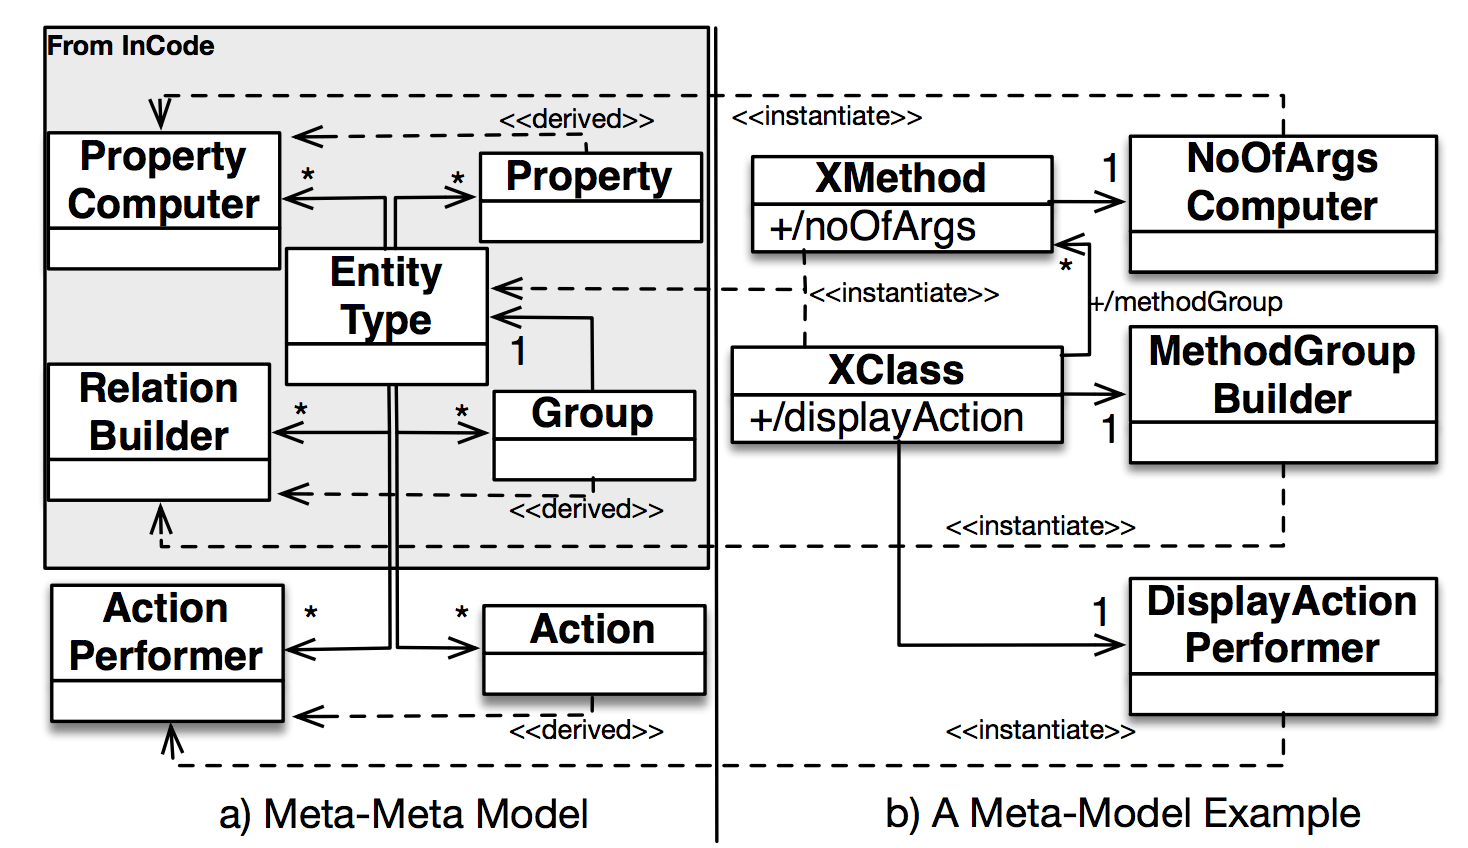
\includegraphics{../img/solution/XMetaModel.png}}
        \caption{XCore meta model \cite{paper:xcore}}
        \label{fig:XMetaModel}
        \end{figure}

\subsection{Interface Component}\label{ch:2.1.2}
        
        When the annotations are processed by the annotation processor, which is presented in chapter \ref{ch:2.1.3}, it will enforce that every concrete type will implement the appropriate
interface. Thus, if the concrete type represents a \textit{property} it must implement a \textit{IPropertyComputer} interface, a \textit{relationship} is expressed by implementing a 
\textit{IRelationshipBuilder} interface and an action requires the \textit{IActionPreformer} interface.

        As we have seen in the section above, a property represents an analysis which is done on an \textit{entity} such as XMethod or XClass from Figure \ref{fig:XMetaModel}. The code below, 
from section \ref{codeSelection:IPropertyComputer}, show how the interface is defined. The code should be self explanatory. The XEntity from the code represent a marker interface for the meta-model entities.
The \textit{ReturnType} can be anything Double, Pair of elements, List of elements, \ldots{} etc.
        
\small
\begin{lstlisting}[language=Java,numbers=left]
 public interface IPropertyComputer <ReturnType, Entity extends XEntity> {
      ReturnType compute(Entity entity);
}   
\end{lstlisting}
\normalsize{} \label{codeSelection:IPropertyComputer}

        In order to express an aggregation relationship between two entities one needs to use the \textit{IRelationshipBuilder} interface \ref{codeSelection:IGroupBuilder}. 
The ElementType \textit{entity} represent the aggregated type and the Entity type represents the aggregator.

\small
\begin{lstlisting}[language=Java,numbers=left]
public interface IRelationshipBuilder <ElementType extends XEntity, Entity extends XEntity> {
    Group<ElementType> buildGroup(Entity entity);
}
\end{lstlisting}
\normalsize{} \label{codeSelection:IGroupBuilder}

        The last interface that can be used is the \textit{IActionPreformer}. As it can be seen from the code \ref{codeSelection:IActionPreformer}, the interface is similar
to the ones presented above. The only major difference is the third type parameter, the ArgTypeList, which is an HList, i.e heterogeneous list. A heterogenous list is a an
arbitrary-length tuple. This means that we can store, in a type safe maner, any numbers of objects, just like in an ordinary list, but the objects do not need to be of the 
same type !

        Our goal is to provide a typesafe maner for building analysis tools. Using an Object array as parameters for the action, though syntacticly convinient, it is by far a dangerous manaer of handling 
such data !

\small
\begin{lstlisting}[language=Java, numbers=left]
public interface IActionPreformer <ReturnType, Entity extends XEntity, ArgTypeList extends IHList> {
  ReturnType performAction(Entity entity, ArgTypeList args);
}

interface IHList {}
public final class HListEmpty implements IHList { } //singleton element
final class HList<HeadType,TailType extends IHList> implements IHList {
  private final HeadType head;
  private final TailType tail;
            
  public HList(HeadType h, TailType t) {
    head = h;
    tail = t;
  }
    
  public HeadType head() {
    return head;
  }

  public TailType tail() {
    return tail;
  }
}
\end{lstlisting}
\normalsize{} \label{codeSelection:IActionPreformer}


\subsection{Annotation Processor}\label{ch:2.1.3}

        In the above sections we presented the syntactic constructs which were employed for the description of the meta-meta-model. But as you have noticed all this construct have additional
semantics, rule of interation, associated to them. In order for them to be fully enforced we have build a compiler plugin, called an \textbf{annotation processor}. The annotation processor
will process only the Java elements that we are interested in, i.e the Java concrete classes annotated with the annotations presented in \ref{ch:2.1.1}. The process of discovering the 
annotated Java element elements is the concer of the Java compiler. As we are a compiler plugin it will invoke us when such elements are found. After all the "interesting" elements 
where processed, the compilation of the project can begin.
        
        Upon processing the elements it will try to see if they respect the following rules \cite{oldThesis}:

        \begin{itemize}
              \item All elements that are annotated must be classes
              \item All annotated classes must have a default constructor.
              \item All elements annotated with @PorpertyComputer must implement
         IPropertyComputer
              \item All elements annotated with @RelationshipBuilder must implement
         IRelationshipBuilder
              \item All elements annotated with @ActionPreformer must implement
         IActionPreformer
              \item  All classes cannot be present in the default package
              \item  The @PropertyComputer, IActionPreformer and @RelationshipBuilder annotations are mutually
        exclusive
              \item  No wildcard types are allowed to be specified for the entity type
         parameter.
            \end{itemize}

        From the known interfaces, IPropertyComputer, IRelationshipBuilder and IActionPreformer, we extract the the meta-model type (i.e the type parameter which extends the XEntity marker interface) 
that is used in that analysis component. For each of the different meta-model types we generate an interface in which every IPropertyComputer / IRelationshipBuilder / IActionPreformer correspond to
a method in the appropriate interface. Of course, to be of any use, the interfaces are fully implemented. The methods from each interface are very easy to implement, they instantiate the concrete "*Computer"
element and call the appropriate method (i.e this is the reason we used interfaces, we have a simple way of guaranteeing the each for this classes have the necessary methods, with the correct definitions). 
The end user has no access to this classes, one can instantiate an entity type (such as XMethod or XClass from Figure \ref{fig:XMetaModel}) by using our provided \textit{Factory}. The factory also includes a cache 
which prevents us from double instantiation of the entities. (this is mostly for performence concers).

        "In Figure \ref{fig:xCoreCommentView} we can see how easily it is for any user to find out which property computers or group builders are implemented for the
entity. The intellisense does all the work. In Figure \ref{fig:xCorexRunExample} we can see an implementation of metric and what code is generated for it by the tool." \cite{oldThesis}

        \begin{figure}
        \centering
        \scalebox{0.3}{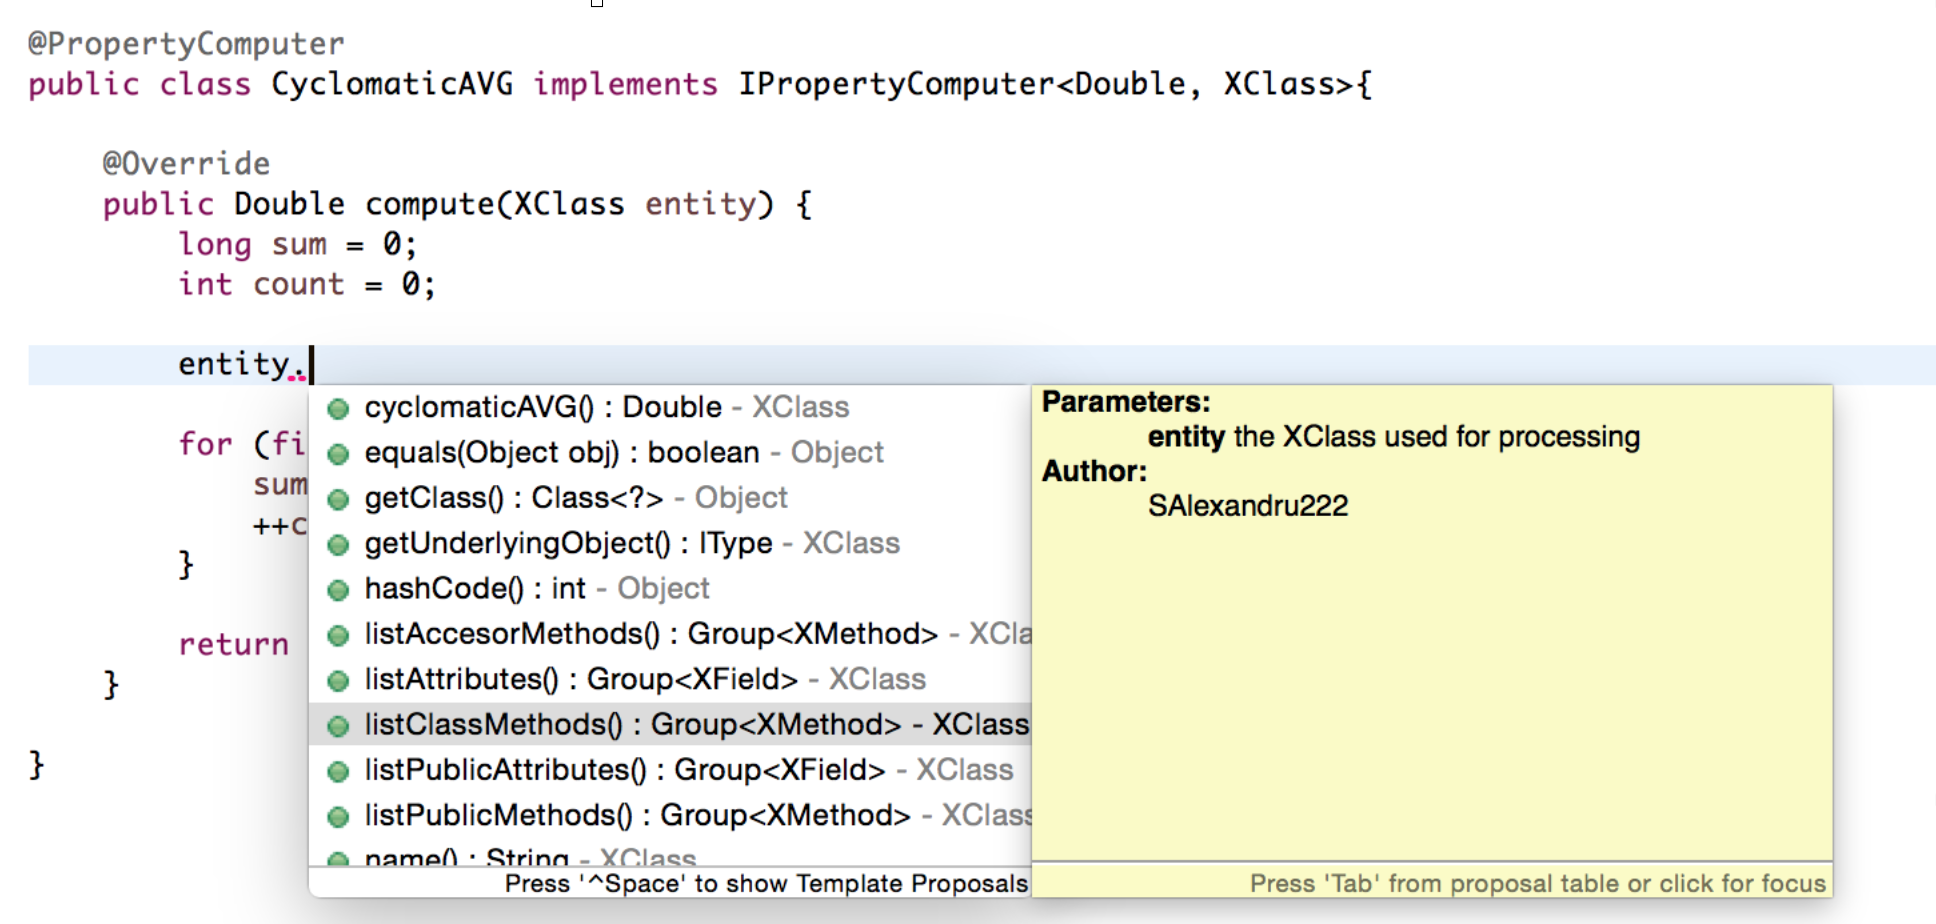
\includegraphics{../img/solution/xCoreCommentView.png}}
        \caption{XCore Intellisense \cite{oldThesis}}
        \label{fig:xCoreCommentView} 
        \end{figure}

        \begin{figure}[ht]
        \centering
        \scalebox{0.25}{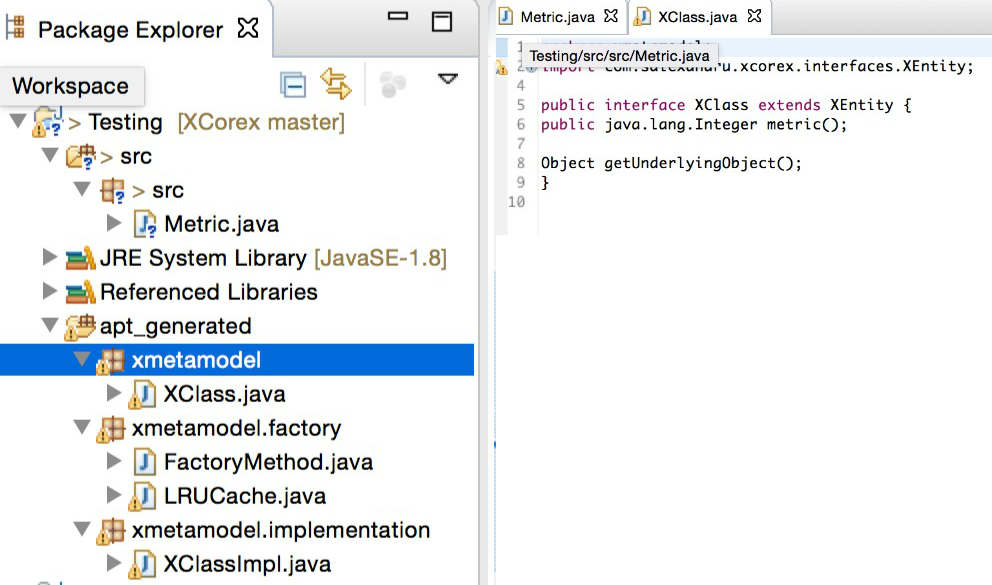
\includegraphics{../img/solution/xCorexRunExample.png}}
        \caption{XCore Type Specification \cite{oldThesis}}
        \label{fig:xCorexRunExample}
        \end{figure}

        From \ref{fig:xCorexRunExample} you should see that the XClass entity, and for that matter any entity from XCore, has an extra method \\ \code{Object getUnderlyingObject}.

        As metioned in Chapter \ref{ch:1} an analysis tool has, at it's core, a back-end which converts the raw project files into meta-model entities. As we have seen in this chapter XCore
provides us with way to describe the meta-mode, but no way of directly extracting it from the raw project files. For this we rely, as most analysis tools actually do, on external 
back-end. It is important to mention that we \textbf{DO NOT} rely on a specific such backend. Thus, each tool deloped with XCore can use its own back-end.
We offer the ability of the developer to choose one, or more such backends and map the back-end entities to our meta-model.
This can be done through the projects configuration page, where we provided a nice type as you go search facility for all the possible types in the project as you can see in figure \ref{fig:xCoreTypeDialogBox}

        \begin{figure}[ht]
        \centering
        \scalebox{0.5}{\rotatebox[origin=c]{90}{{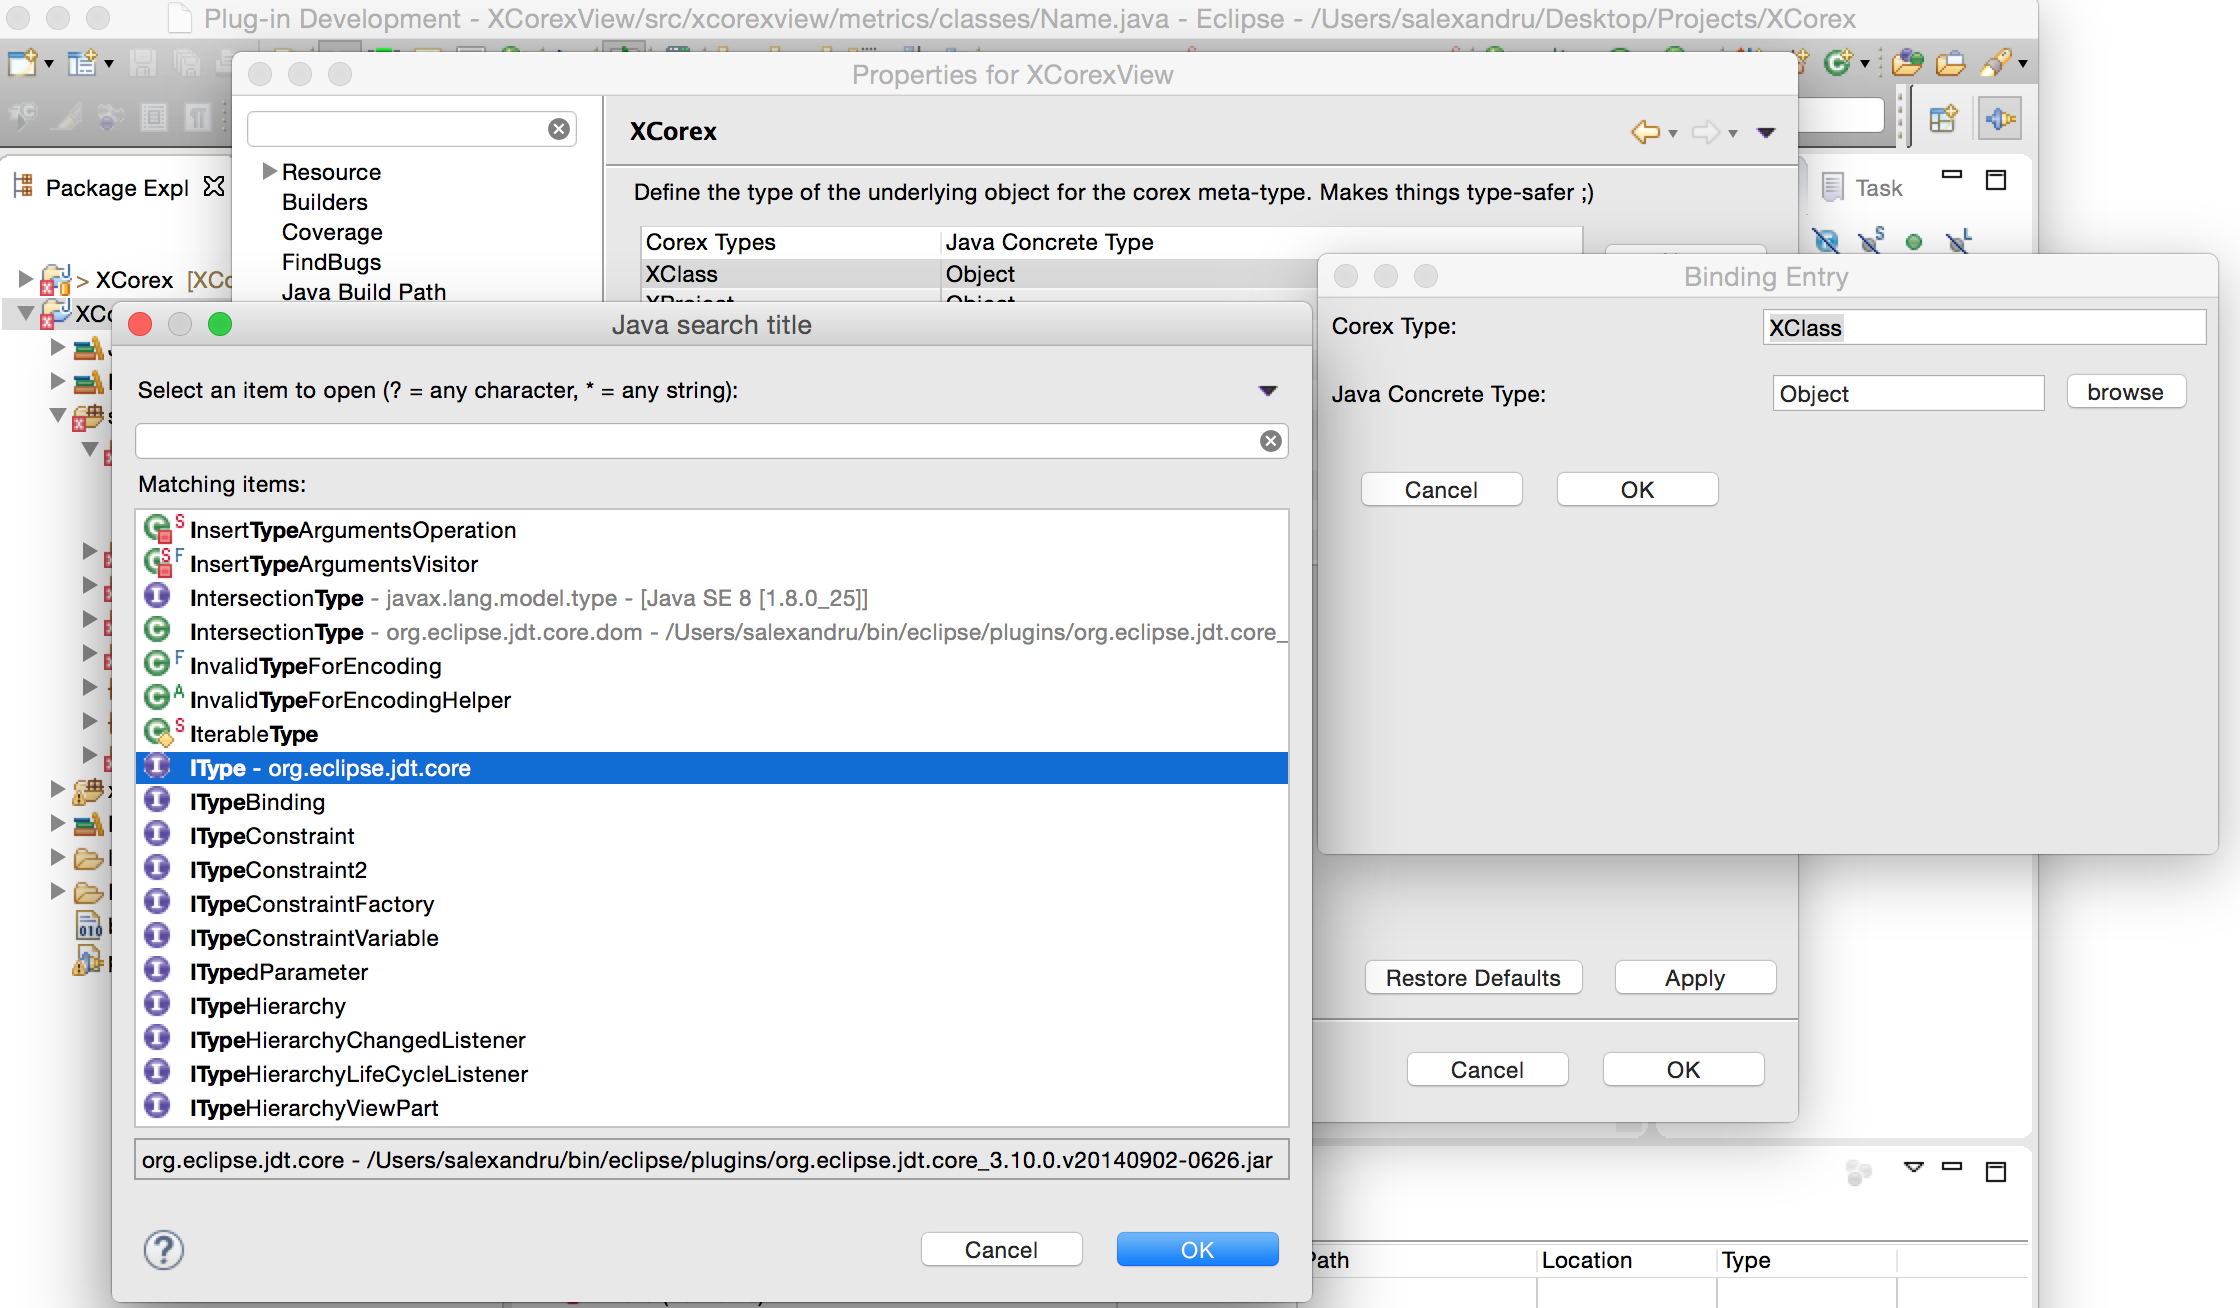
\includegraphics{../img/solution/xCoreTypeDialogBox.png}}}}
        \caption{XCore Type Dialog Box \cite{oldThesis}}
        \label{fig:xCoreTypeDialogBox}
        \end{figure}


\subsection{Connection to Multiple Back-ends}

        The user has the ability to specify, to map if you wish, the abstract XCore entities (like XClass and XMethod from above) to concrete entities that are extracted by a back-end. For example we
could map an XClass to an IType from Eclipse JDT and XMethod to an IMethod. How this is done by the devloper is presented in the section below.

        What happens behind the secene is that for each XClass entity we generate an interface with the same name and it's coresponding implementation as can be seen in Figure \ref{fig:xCorexRunExample}.
For each of this elements we provide an accessor method called \code{getUnderlyingObject} which returns the corresponded object extracted by the back-end. In order to provide the reverse maping we offer
a Factory of XEntities which uses the the concrete entities (i.e IType and IClass) to instantiate the XClass and XMethod entities.

        Sometimes using just one back-end isn't enough. We may one to integrate two tool which use different back-ends, or simply our current back-end isn't offering all the tools we need to implement 
what we need and may want to integrate with another back-end to complement it. Whatever the reason, we can know integrate more than one back-end into XCore.  

        This is done by providing a trasformer, i.e a class that extends \code{ITrasnform} interface, and which can transform an element from one back-end to another back-end and reverse. It is the job
of the developer to provide this element. Once provided our tool can generate similar method to \code{getUnderlyingObject} which allow the developers to switch from one representation to another.

\subsection{Tool extension}

	This feature has a nice analogy in Object Oriented Programming, i.e Inheritence. We have base-tool which a sub-tool that we have implemented will extend. 

	This is done so we can improve the functionality of the base-tool and also be able to add new features to it, without breaking the original developed tool. It works by copying the 
entire base-tool project into the sub-tool project. This ensures that we have all the needed dependencies. After we have copied the code, we have to make sure that the entities have the 
appropriate concrete type mapped. This is done by adding, yet another concept, \textit{extended underlying type}. This is set during this process and cannot be altered. Also, once this
type is set we cannot change the underlying object.
        

